\section{Innovation Is a Game}\label{sec:game}
% Reader question: Can invention be played like Go?
% Core points advanced: 1 (primary: innovation is a game), 2 (novelty is free;
% judgment is the inventor), 3 (search = 1)
% Exhibits: Table 4 (tab:go-vs-innovation), Figure 3 (fig:game-loop)

We define one attempt at algorithm invention as a game: the encoded
problem is the board, a program is the move, the referee checks and
scores it, and a declared incumbent is the opponent.

Encoding the problem
provides a shared interface; each task type still needs its own qualified
encoding, language and evaluation protocol (\cref{sub:game-boards}).


% ----------------------------------------------------------------------------
\subsection{Why games came first}\label{sub:game-games}

Games became AI's laboratory because they supply four things at once: fixed
rules, an impartial referee, a clear winner and cheap replay. Chess was chosen
because it is ``sharply defined both in allowed operations (the moves) and in
the ultimate goal (checkmate)'' \citep{shannon1950chess}, and checkers showed
that a program could improve by playing itself \citep{samuel1959checkers}.

Together these properties support repeated, reproducible evaluation. People
scale judgment the same way, through prizes, leaderboards and the common task
framework's ``scoring referee'' \citep{donoho2017fifty} (\cref{sec:road}).
Invention has the first three properties once the problem and the solution are
written down, within the limits of \cref{sub:game-played}; cheap replay is a
question of cost (\cref{sec:price}).

% ----------------------------------------------------------------------------
\subsection{The rules}\label{sub:game-rules}

\Cref{tab:go-vs-innovation} sets the game beside Go. An illegal move is
counted as a failed attempt. The reference writer reads the encoded problem.
The referee keeps the incumbent as a separate comparison standard
(\cref{sub:method-board}); its code and score must stay outside the writer's
input.

\begin{table}[!htb]
  \caption{\textbf{Go and the innovation game, element by element.}
  Moves differ most: Go's are cheap, while each program is costly to judge
  (\cref{sub:game-played}). Go's game length is
  from \citet{silver2016mastering}.}
  \label{tab:go-vs-innovation}
  \centering
  \small
  \setlength{\tabcolsep}{4pt}
  \setlength{\extrarowheight}{2pt}% separates rows whose cells wrap
  \begin{tabular}{@{}>{\raggedright\arraybackslash}p{0.18\linewidth}>{\raggedright\arraybackslash}p{0.32\linewidth}>{\raggedright\arraybackslash}p{0.42\linewidth}@{}}
    \toprule
                   & Go                              & The innovation game \\
    \midrule
    Board          & Stones on a $19\times19$ grid   & The encoded problem \\
    Move           & Place one stone, or pass        & Write one complete program \\
    Legal move     & Empty point; no suicide or forbidden repetition & Parses, type-checks, runs within limits \\
    Illegal move   & Not allowed                     & Stillborn: an automatic loss \\
    Referee        & The rules of Go                 & The verifier, on hidden folds \\
    Win            & Higher final score             & Valid, and beats the incumbent \\
    Opponent       & A past self                     & The incumbent, often a past self \\
    Rating         & Elo                             & Win rate and Elo across problems \\
    Moves per game & About 150, each cheap           & One, costly to judge \\
    \bottomrule
  \end{tabular}
\end{table}
% Figure 3 is defined here, ahead of its first reference, so that the
% full-width float can reach the top of the page where it is cited.
\begin{figure*}[t]
  \centering
  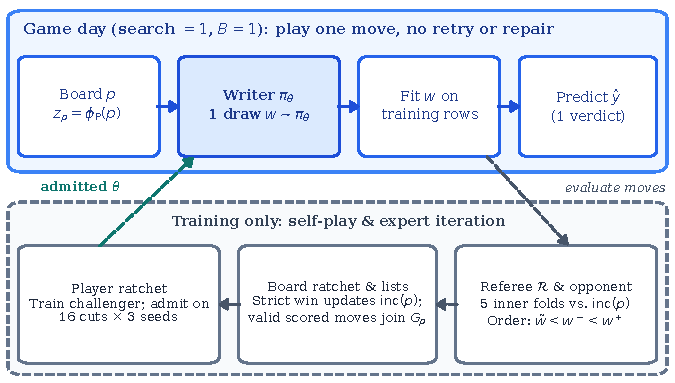
\includegraphics[width=\textwidth]{figures/fig3_game_loop.pdf}
  \caption{\textbf{Training plays the whole game; game day plays one move.}
  Schematic. Top row (blue): game day. Dashed box: training only. Outcomes
  are recorded; valid scored programs can enter the learning lists, while
  failed attempts still count against the budget.}
  \label{fig:game-loop}
\end{figure*}

Formally, the game is a tuple of seven parts,
\[
  \Game = (\Prob, \encP, \Sol, \encS, \referee, \reward, \opp).
\]
Here $\encP$ and $\encS$ embed a problem $p \in \Prob$ and a program
$w \in \Sol$ as $z_p$ and $z_w$. The referee $\referee$ reports a program's
validity and score, the reward $\reward$ orders moves, and the opponent $\opp$
supplies the incumbent $\inc{p}$. The tuple extends Rice's model of algorithm
selection \citep{rice1976algorithm}: the player writes the algorithm instead of
picking it, and a declared incumbent sets the comparison standard.

With one move, the game is a contextual bandit: the board supplies context,
the program is the action and the
verdict is the reward \citep{lattimore2020bandit}. It earns the name through an
opponent that improves as the player does. The asymmetry is in the
moves: Go offers about 250 legal moves per turn over about 150 turns, each free
to check \citep{silver2016mastering}, while this game offers one move, costly to
judge. Under a single-attempt budget, the chance $\winprob$ of a win matters
directly (\cref{eq:taste}). Whether training raises that chance on new
families is the test in \cref{sec:results}.

\Cref{fig:game-loop} draws the loop. Game day plays only its top row, so
nothing can send a move back for another try; that is \searchone.

% ----------------------------------------------------------------------------
\subsection{The board and the move}\label{sub:game-board}

The board is the aim pillar of \cref{sec:anatomy}, made machine-readable: a
summary of the training data, the objective and metric, and the constraints.
Landmark scores from cheap learners \citep{pfahringer2000landmarking} and
learned tabular summaries are possible encodings. The reference checkpoint
in \cref{sub:method-board} uses a frozen 2,048-value summary with a
30-second cap.
A useful board should preserve distinctions relevant to algorithm choice,
remain stable under irrelevant reorderings, exclude final evaluation
information and have a measured cost. These are requirements to test, not
properties guaranteed by naming an encoder. People still choose the problem
and define what counts as a useful solution.

A move is one program in a typed language over learning primitives.
The reference language uses a 401-token
vocabulary, with up to six transforms chosen from 31 and one of 22 prediction
heads (\cref{sub:method-move}).

Types remove whole classes of stillborn
programs before they run \citep{montana1995stgp}. Canonicalization can merge
syntactic variants; it need not identify every functionally equivalent
implementation. AutoML-Zero
reused scores when hashes of truncated predictions matched after a short
training and validation probe \citep{real2020automlzero}. Matching a probe
does not establish agreement on other inputs (\cref{sub:method-move}).

The language bounds what can be expressed; changing its primitives changes
that space \citep{boden1990creative}. The reference grammar also bounds
composition depth. Structural constraints can prevent invalid programs; their effect on useful proposal
quality must be measured (\cref{sec:results}).

% ----------------------------------------------------------------------------
\subsection{The referee and the opponent}\label{sub:game-referee}

The reward is an ordering first and a number second. Validity is a gate: any
stillborn program scores below any valid one. Past the gate, programs rank by
improvement over the incumbent on hidden folds. The reference promotion
rule keeps the existing incumbent on a tie. Novelty never pays for losing: any novelty
bonus (\cref{sec:price}) must respect the order. For a stillborn program
$\tilde{w}$, an also-ran $w^-$ and a win $w^+$ on board $p$,
\[
  \reward(p, \tilde{w}) \;<\; \reward(p, w^-) \;<\; \reward(p, w^+).
\]

The opponent is a ratcheting incumbent. In the reference procedure, only
strict improvement on five inner folds under the same evaluation protocol
can displace a board's incumbent.
A retrained writer has a separate
admission test on 16 held-out cuts with three seeds each
(\cref{sub:method-selfplay}). Together the two ratchets make this self-play:
the player keeps facing a standard often set by its own earlier play.
AlphaGo Zero likewise separated network admission from choosing a move
during play \citep{silver2017mastering}.

Subtracting the incumbent's score does not change which move is best.
Promotion raises the bar, turns yesterday's winners
into today's also-rans and shifts which problems are worth playing. The
reference learning targets use each program's rank within its scored list
(\cref{sub:method-map,sub:method-selfplay}).

% ----------------------------------------------------------------------------
\subsection{One game, many boards}\label{sub:game-boards}

Binary and multiclass classification, regression, ranking, forecasting and
relational prediction are prospective boards. A shared formal interface
still needs a compatible encoding, program language, metric and validation
protocol qualified for each task type.

Beyond machine learning, examples of referees include sorting tests
\citep{mankowitz2023alphadev}, evaluators for mathematical constructions
\citep{romeraparedes2024funsearch} and accelerator-kernel timers
\citep{novikov2025alphaevolve}. These motivate extensions of the recipe,
rather than results of this paper (\cref{sec:meaning}).

Casting algorithm discovery as a game is not new, but earlier games wrote one
family of problems into their rules, as AlphaTensor did for matrix
multiplication and AlphaDev for sorting
\citep{fawzi2022alphatensor,mankowitz2023alphadev}. AlphaZero used one algorithm
for three games and trained a separate network for each
\citep{silver2018general}. Here the problem is an input on the board, so one
player can, in principle, learn many boards.

\begin{keyidea}
A reliable referee makes a discipline a candidate for this game; transfer
to that discipline still needs evidence.
\end{keyidea}

% ----------------------------------------------------------------------------
\subsection{The analogy's limits}\label{sub:game-played}

A worked game, chosen by a rule fixed before inspection, is to be reported with
the results (\cref{sub:results-failures}). The analogy breaks in four places.

\textbf{The referee is noisy}: picking a
winner by a noisy validation score biases that score upward
\citep{cawley2010overfitting}. Strict numerical improvement alone does not
quantify confidence; independent evaluation and an uncertainty protocol are
needed to interpret it.

\textbf{Moves are expensive}, each a fit and a cross-validation
(\cref{sec:price}).

\textbf{Judges can be gamed}, as METR documented for
frontier models in June 2025 \citep{metr2025rewardhacking}; \cref{sec:method}
lists our safeguards.

And \textbf{no algorithm wins everywhere}: averaged
uniformly over all problems, no learner has lower error off the training set
than another, ours included \citep{wolpert1996nfl}.

Real problems are structured, though, and a player that
reads the board can choose its bias board by board. \Cref{sec:results} reserves the tests of that hypothesis against fixed
frontier-designed algorithms, with paired outcomes beside Elo summaries
\citep{elo1978rating}. Non-transitive comparisons are one reason not to
reduce the evidence to a single rating \citep{balduzzi2018reevaluating}.

Those rules define an attempt. Pricing a verified improvement must also
count attempts that fail or lose.
